\documentclass[12pt]{article}

%AMS-TeX packages
\usepackage{amssymb,amsmath,amsthm} 
%geometry (sets margin) and other useful packages
\usepackage[margin=1.25in]{geometry}
\usepackage{graphicx,ctable,booktabs}


%Redefining sections as problems
%
\makeatletter
\newenvironment{problem}{\@startsection
       {section}
       {1}
       {-.2em}
       {-3.5ex plus -1ex minus -.2ex}
       {2.3ex plus .2ex}
       {\pagebreak[3]%forces pagebreak when space is small; use \eject for better results
       \large\bf\noindent{Problem }
       }
       }
       {%\vspace{1ex}\begin{center} \rule{0.3\linewidth}{.3pt}\end{center}}
       \begin{center}\large\bf \ldots\ldots\ldots\end{center}}
\makeatother


%
%Fancy-header package to modify header/page numbering 
%
\usepackage{fancyhdr}
\pagestyle{fancy}
%\addtolength{\headwidth}{\marginparsep} %these change header-rule width
%\addtolength{\headwidth}{\marginparwidth}
\lhead{Problem \thesection}
\chead{} 
\rhead{\thepage} 
\lfoot{\small\scshape CS124} 
\cfoot{} 
\rfoot{\footnotesize PA 1 Writeup} 
\renewcommand{\headrulewidth}{.3pt} 
\renewcommand{\footrulewidth}{.3pt}
\setlength\voffset{-0.25in}
\setlength\textheight{648pt}

%1%%%%%%%%%%%%%%%%%%%%%%%%%%%%%%%%%%%%%%%%%%%%%%

%
%Contents of problem set
%    

\title{CS 124 - Programming Assignment 2}
\author{Aidan Daly and Willie Yao}
\usepackage{fullpage}
\usepackage{graphicx}
\usepackage{epstopdf}

\begin{document}
\maketitle

\begin{problem}{}
\textbf{Implementation details and optimizations}\\
\\
We decided to represent our matrices as two-dimensional arrays of integers, and wrote helper functions for allocating and freeing them. \\
Random matrices for all tests were created such that each entry was uniformly random between 0, 1, and 2, though we also have support for testing under several other random integer schemes.\\
\\
\textbf{Conventional algorithm}

We decided to improve upon the efficiency of the conventional algorithm by using a more cache-friendly approach.  For a matrix multiplication of $A \times B$, the most naive method would iterate through the rows of $A$ and the columns of $B$, taking the dot product of each pair of vectors.  This approach would cause a lot of cache misses, however, as two-dimensional arrays in C are stored in row-major order.  This would mean $A$ would have no problem iterating through any row of the array, as the whole row will be loaded into the cache after the first miss, while iterating through a column of $B$ would result in a cache miss and a call to memory on every iteration.

To make our implementation more efficient, we wrote a helper function that would take a pointer to a square matrix and transpose it.  Thus, when multiplying $A \times B$, we would transpose $B$, iterate through $A$ and $B$ in row-major order, and dot product each pair of rows.  This minimized caches misses and greatly improved performance, as shown in the figure below:
\begin{center}
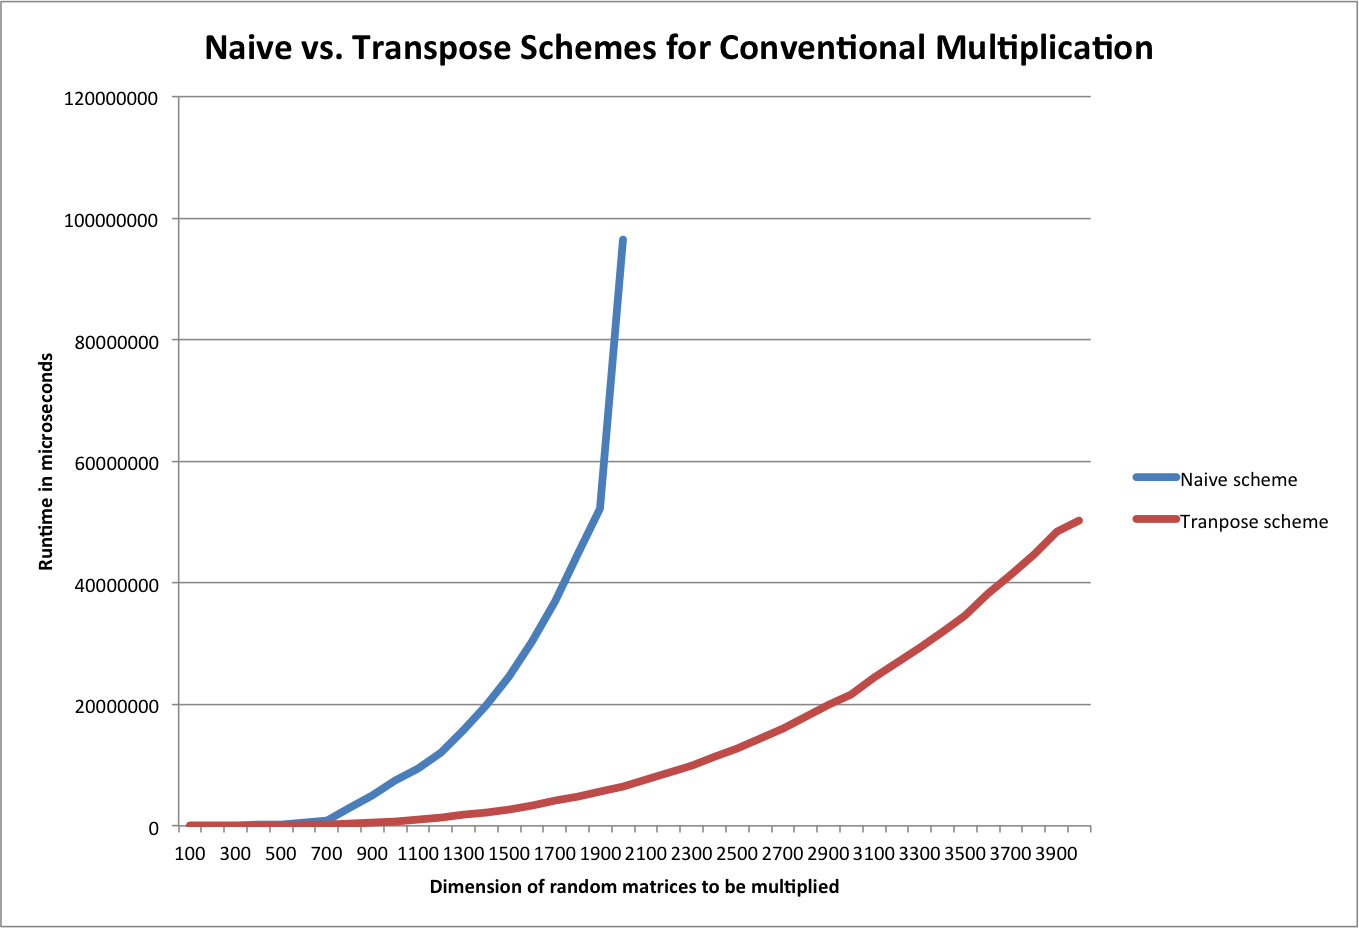
\includegraphics[scale=.70]{figs/conventional.png}
\end{center}
\textbf{Strassen's algorithm}

Because Strassen's algorithm must operate on even matrices, at every level of recursion, it will only run all the way to a base case on square matrixes of a dimension that is some power of 2.  Thus, to account for matrices that are not a power of two, we had two options: 1) pad the matrices with zeroes up front such that their dimension will reach a power of two, or 2) pad up to an even dimension whenever an odd one comes up in the recursion.  

We opted for up-front padding because it would call for the least memory copying at the expense of a worst case of nearly doubling the dimension of a matrix up front (if its dimension is slightly larger than a power of two).  Thus, our matrices are allocated with dimension equal to the closest upper power of two and padded with zeroes before being populated with either data from a text file or random integers.\\

We made two important optimizations in the recursion portion of Strassen's algorithm that avoided unnecessary memory allocation and copying.  The first one has to do with the splitting of the even-dimensioned, square matrix into four sub matrices.  A naive approach would be to allocate four appropriately size matrices, copy the relevant data into them, then recurse on them and free afterwards.  This causes quite a bit of  overhead at each step.

To circumvent this, we took advantage of the "dimension" parameter that we pass to our recursive function for Strassen, which gets halved at each level.  If we think of a matrix as being divided into quadrants:
\begin{center}
$A11 | A12$\\
$----$\\
$A21 | A22$
\end{center}
We can access quadrants $A11$ and $A21$ by simple pointer arithmetic and an updated bound on the dimension.  We pass pointers into the original matrix $A$ along with a bound and avoid copying data, since none of the functions in Strassen's algorithm alter the original matrices.  As for quadrants $A12$ and $A22$, we had to allocate temporary matrices and copy over the relevant data, because we can't easily make "slices" of matrix rows the way we can with columns, due to row-major ordering of matrices.   Still, this cut temporary memory allocation and copying in half.\\

Our second memory optimization involved storing the intermediate results [WILLIE - talk about your functions] \\

Lastly, because the worst-case scenario of Strassen's involves almost doubling the size of the original matrix, we decided to pass extra parameters to our Strassen function that would serve as the "coordinates" of the sub matrix in our original matrix.  For example, $A11$ would have coordinates (0,0) and $A12$ would have coordinates (0,$\frac{dim}{2}$).  Knowing these coordinates, the current problem dimension, and the original dimension before padding, the algorithm can know immediately if it is operating on a zero matrix from the madding, and instantly return a zero matrix without recursing further.  When Strassen operates on matrices like $A11+A22$, the minimum of the coordinates between the two matrices is passed, since the resulting matrix is relevant and should be recursed on if any of its components were non-padding.  This optimization eliminates many unnecessary recursive steps in over padded matrices.

\end{problem}{}

\begin{problem}{}
Analytical work\\

\end{problem}{}
\begin{problem}{}
Experimental work\\

To experimentally determine the optimum cutoff value for Strassen's algorithm, we decided to run the algorithm on random matrices of dimension 4097 and compare the runtimes with different cutoff values.  We chose the problem dimension as 4097 because it is a relatively large number and also is one greater than a power of two.  This gives us a "worst case" runtime scenario for Strassen's algorithm, since it must pad this matrix to the next closest power of two - 8192.

After experimenting with a wide range of cutoff values (from 100 to 4000 in increments of 100), we obtained the graph below:
\begin{center}
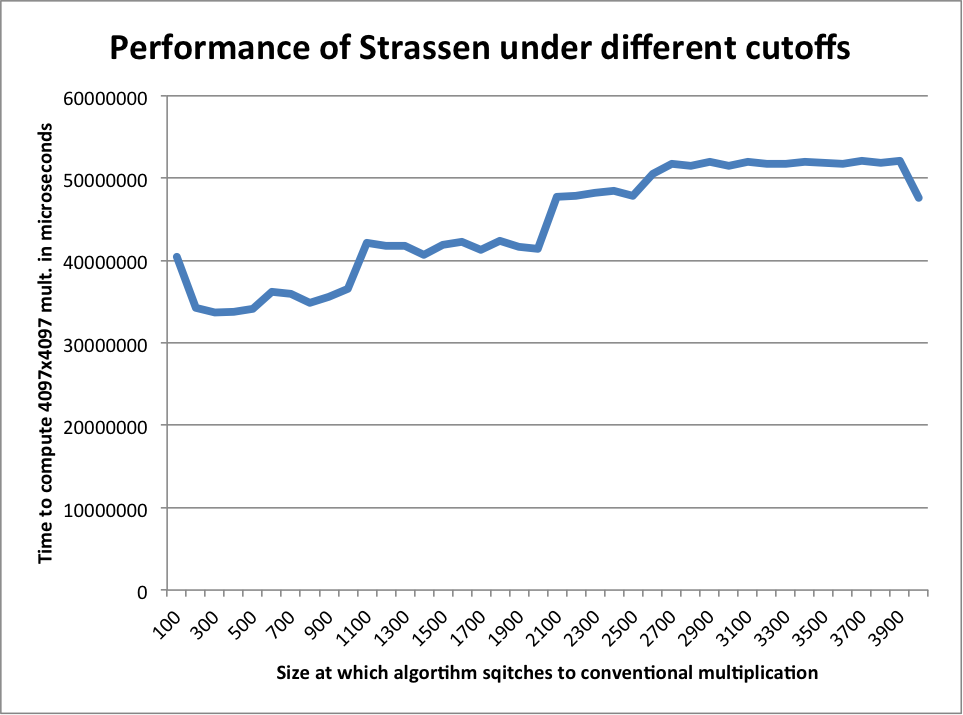
\includegraphics[scale=0.8]{figs/benchmark-1.png}
\end{center}

This allowed us to refine our guess to be somewhere in the 100 to 1000 range.  Because our implementation of Strassen's algorithm only operates on matrices whose dimensions are powers of 2, we extensively tested the algorithm against 4097x4097 random matrix multiplications with cutoffs of $\{64, 128, 256, 512, 1024\}$.  The results for these tests are shown below:
\begin{center}
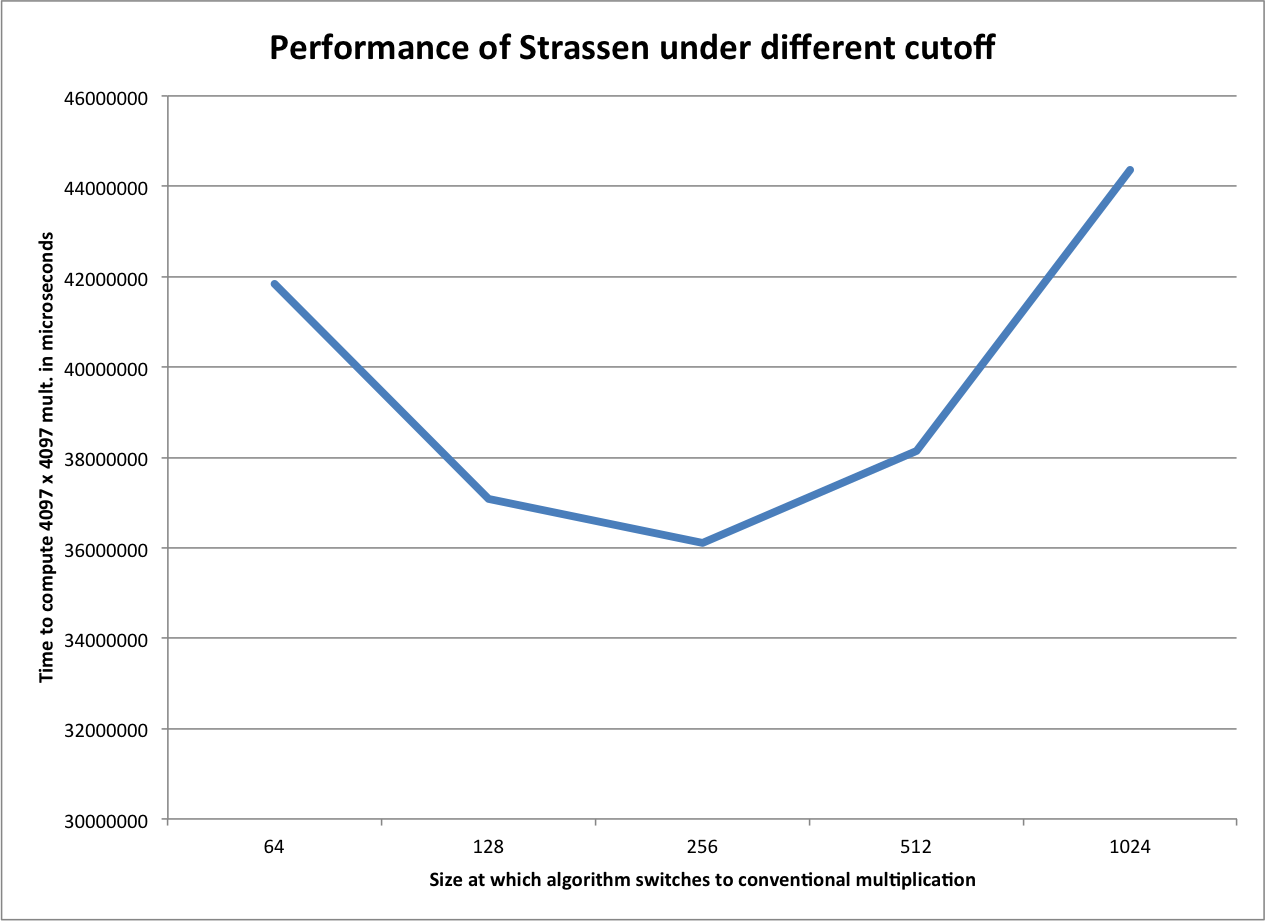
\includegraphics[scale=0.75]{figs/benchmark-2.png}
\end{center}

Thus, through our experimental work we have determined that the optimal cutoff for out implementation of Strassen's algorithm to switch over to the transpose-conventional implementation is 256.
\end{problem}{}

\end{document}